% Graphical abstract for systems-4669426 (revision).
%
% MDPI house rule: graphical content only. No article title, authors, affiliations or
% citation line. Palette = the paper's figure palette (make_revision_figures.py):
% blue #2a78d6, orange #eb6834, aqua #1baf7a, ink #0b0b0b, muted #52514e, grid #d9d8d4.
%
% Numbers (all from pva-experiments v0.5.0, experiments/results/):
%   panel 1  audit/audit_summary.csv, published settings (NSGA-II, 150 generations):
%            exact optimum 74.6 / 85.2, committed evolutionary decision 97.4 / 120.7
%            (small / large, equal weights, lower is better); 97-100% of front points dominated.
%   panel 2  seed floor 83-94% churn (audit_summary churn_floor, published settings);
%            within 1% of the optimum 26-33% (multiplicity/summary.csv);
%            tie-break: 10 plain solves -> 10 optima, stated rule -> 1 (multiplicity/tiebreak.csv).
%   panel 3  turbulence_extended/summary.csv, large size, median regret over 36 conditions;
%            joint/sum of parts 0.78 at level 0.4.
% Render: pdflatex graphical-abstract.tex && pdftoppm -png -r 300 -singlefile graphical-abstract.pdf graphical-abstract
\documentclass[border=0pt]{standalone}
\usepackage[T1]{fontenc}
\usepackage{tgheros}
\renewcommand{\familydefault}{\sfdefault}
\usepackage{pgfplots}
\pgfplotsset{compat=1.18}
\usetikzlibrary{positioning,arrows.meta,calc}

\definecolor{gblue}{HTML}{2A78D6}
\definecolor{gorange}{HTML}{EB6834}
\definecolor{gaqua}{HTML}{1BAF7A}
\definecolor{gink}{HTML}{0B0B0B}
\definecolor{gmuted}{HTML}{52514E}
\definecolor{ggrid}{HTML}{D9D8D4}
\definecolor{gpaper}{HTML}{FAFAF8}

\pgfplotsset{
  gaxis/.style={
    axis line style={gmuted}, tick style={gmuted}, ticklabel style={text=gmuted, font=\fontsize{8}{9}\selectfont},
    label style={text=gink, font=\fontsize{8.5}{10}\selectfont},
    major grid style={ggrid}, ymajorgrids,
    /pgf/number format/assume math mode=true,
    axis x line*=bottom, axis y line*=left,
  }
}

\begin{document}
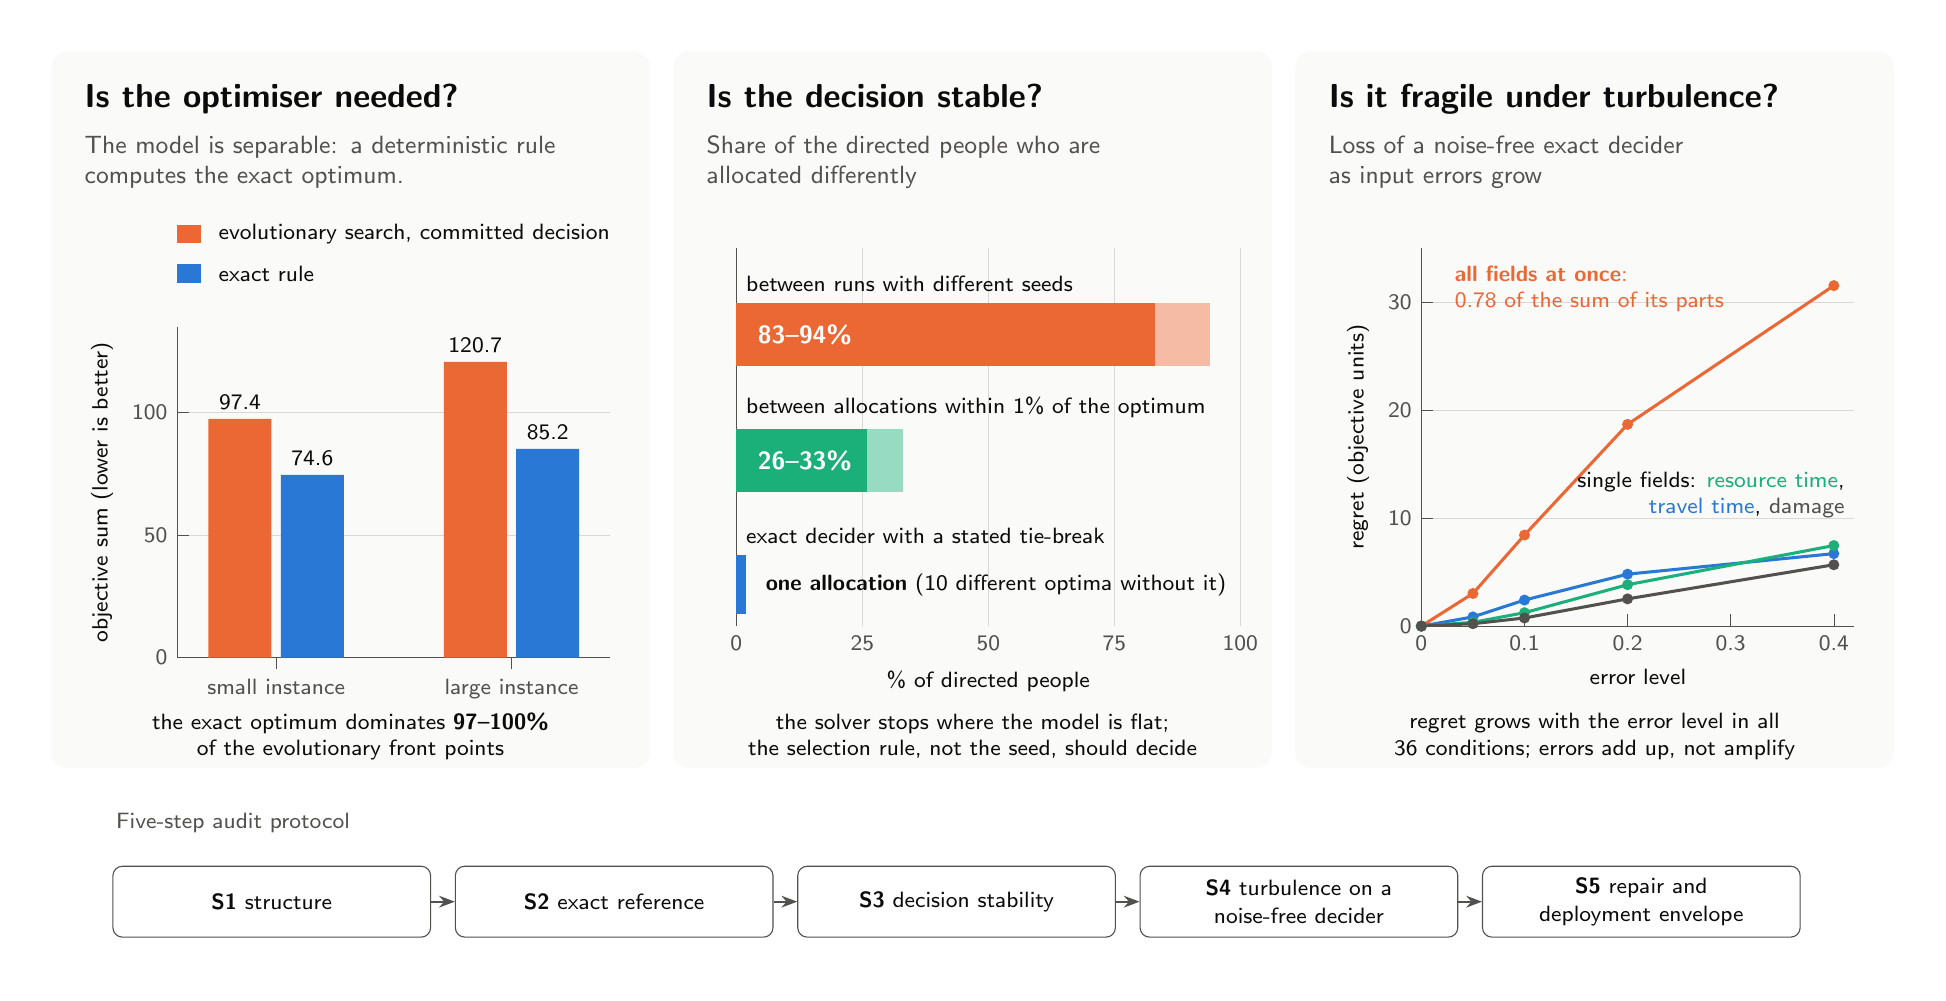
\begin{tikzpicture}[x=1mm,y=1mm,
  q/.style={anchor=north west, text=gink, font=\bfseries\fontsize{13}{15}\selectfont},
  ans/.style={anchor=north west, text=gmuted, align=left, font=\fontsize{9}{11}\selectfont, text width=70mm},
  note/.style={text=gink, font=\fontsize{8}{9.6}\selectfont, align=center},
  stp/.style={draw=gmuted, fill=white, rounded corners=1.2mm, minimum height=9mm, text width=38mm,
               align=center, font=\fontsize{8.4}{10}\selectfont, text=gink, line width=0.4pt},
]
\fill[white] (0,0) rectangle (240,120);

% ---------- panel frames ----------
\foreach \x in {3,82,161} {
  \fill[gpaper, rounded corners=2mm] (\x,26) rectangle ++(76,91);
}

% ================= Panel 1: necessity =================
\node[q] at (6,114) {Is the optimiser needed?};
\node[ans] at (6,107.5) {The model is separable: a deterministic rule\\computes the exact optimum.};
\fill[gorange] (19,92.6) rectangle ++(3,2.4); \node[note, anchor=west] at (23,93.8) {evolutionary search, committed decision};
\fill[gblue] (19,87.6) rectangle ++(3,2.4); \node[note, anchor=west] at (23,88.8) {exact rule};
\begin{axis}[gaxis, scale only axis, at={(19mm,40mm)}, width=55mm, height=42mm,
  ybar=1.2mm, bar width=8mm, ymin=0, ymax=135, ytick={0,50,100},
  symbolic x coords={small,large}, xtick=data, enlarge x limits=0.42,
  xticklabels={small instance, large instance},
  ylabel={objective sum (lower is better)},
  nodes near coords, every node near coord/.append style={font=\fontsize{8}{9}\selectfont, text=gink},
  ]
  \addplot[fill=gorange, draw=none] coordinates {(small,97.4) (large,120.7)};
  \addplot[fill=gblue, draw=none] coordinates {(small,74.6) (large,85.2)};
\end{axis}
\node[note] at (41,30) {the exact optimum dominates \textbf{97--100\%}\\of the evolutionary front points};

% ================= Panel 2: decision stability =================
\node[q] at (85,114) {Is the decision stable?};
\node[ans] at (85,107.5) {Share of the directed people who are\\allocated differently};
\begin{scope}[shift={(90,0)}]
  % axis: 0..100 % over 64 mm
  \foreach \t in {0,25,50,75,100} {
    \draw[ggrid] ({\t*0.64},44) -- ({\t*0.64},92);
    \node[text=gmuted, font=\fontsize{8}{9}\selectfont, below] at ({\t*0.64},44) {\t};
  }
  \node[note, below] at (32,39.5) {\% of directed people};
  \draw[gmuted] (0,44) -- (0,92);
  % between seeds: 83-94
  \node[note, anchor=south west] at (0,85.2) {between runs with different seeds};
  \fill[gorange] (0,77) rectangle ({83*0.64},85);
  \fill[gorange!45] ({83*0.64},77) rectangle ({94*0.64},85);
  \node[anchor=west, text=white, font=\bfseries\fontsize{9}{10}\selectfont] at (1.5,81) {83--94\%};
  % within 1% of optimum: 26-33
  \node[note, anchor=south west] at (0,69.2) {between allocations within 1\% of the optimum};
  \fill[gaqua] (0,61) rectangle ({26*0.64},69);
  \fill[gaqua!45] ({26*0.64},61) rectangle ({33*0.64},69);
  \node[anchor=west, text=white, font=\bfseries\fontsize{9}{10}\selectfont] at (1.5,65) {26--33\%};
  % tie-break
  \node[note, anchor=south west] at (0,53.2) {exact decider with a stated tie-break};
  \fill[gblue] (0,45.5) rectangle (1.2,53);
  \node[note, anchor=west, align=left] at (2.5,49.2) {\textbf{one allocation} (10 different optima without it)};
\end{scope}
\node[note] at (120,30) {the solver stops where the model is flat;\\the selection rule, not the seed, should decide};

% ================= Panel 3: input fragility =================
\node[q] at (164,114) {Is it fragile under turbulence?};
\node[ans] at (164,107.5) {Loss of a noise-free exact decider\\as input errors grow};
\begin{axis}[gaxis, scale only axis, at={(177mm,44mm)}, width=55mm, height=48mm,
  xmin=0, xmax=0.42, ymin=0, ymax=35, xtick={0,0.1,0.2,0.3,0.4}, ytick={0,10,20,30},
  xticklabels={0,0.1,0.2,0.3,0.4},
  xlabel={error level}, ylabel={regret (objective units)},
  every axis plot/.append style={line width=1.1pt, mark size=1.4pt},
  ]
  \addplot[gorange, mark=*] coordinates {(0,0) (0.05,3.02) (0.1,8.43) (0.2,18.68) (0.4,31.53)};
  \addplot[gblue, mark=*] coordinates {(0,0) (0.05,0.85) (0.1,2.41) (0.2,4.81) (0.4,6.71)};
  \addplot[gaqua, mark=*] coordinates {(0,0) (0.05,0.35) (0.1,1.24) (0.2,3.83) (0.4,7.46)};
  \addplot[gmuted, mark=*] coordinates {(0,0) (0.05,0.22) (0.1,0.75) (0.2,2.52) (0.4,5.68)};
\end{axis}
\node[note, anchor=north west, text=gorange, align=left] at (180,91) {\textbf{all fields at once}:\\0.78 of the sum of its parts};
\node[note, anchor=south east, align=right] at (232,56.5) {single fields: {\color{gaqua}resource time},\\{\color{gblue}travel time}, {\color{gmuted}damage}};
\node[note] at (199,30) {regret grows with the error level in all\\36 conditions; errors add up, not amplify};

% ================= bottom strip: the protocol =================
\node[anchor=west, text=gmuted, font=\fontsize{8.5}{10}\selectfont] at (10,19) {Five-step audit protocol};
\node[stp] (s1) at (31,9) {\textbf{S1} structure};
\node[stp, right=3mm of s1] (s2) {\textbf{S2} exact reference};
\node[stp, right=3mm of s2] (s3) {\textbf{S3} decision stability};
\node[stp, right=3mm of s3] (s4) {\textbf{S4} turbulence on a\\noise-free decider};
\node[stp, right=3mm of s4] (s5) {\textbf{S5} repair and\\deployment envelope};
\foreach \a/\b in {s1/s2,s2/s3,s3/s4,s4/s5} \draw[-{Stealth[length=2mm]}, gmuted, line width=0.6pt] (\a) -- (\b);
\end{tikzpicture}
\end{document}
